\chapter{OpenCAL}

With the name OpenCAL, we identify the sequential version of the
software library, which runs on just a single core of your CPU. It
represents the basis for the other parallel versions. Moreover, it
allows for some \emph{unsafe operations}, which can significantly speed up
your application. Such unsafe operation can also be found in the
OpenMP version, while they are not present to GPU one.

In the following sections, we will introduce OpenCAL by examples. In
the first part of the Chapter, we will deal with the OpenCAL's safe
mode, while in the last one, we will go deep inside OpenCAL,
discussing unsafe operations.

\section{Conway's Game of Life}

In order to introduce you to Cellular Automata development with
OpenCAL, we start this section by implementing the Conway's Game of
Life. It represents one of the most simple, yet powerful examples of
Cellular Automata, devised by the mathematician John Horton Conway in
1970.

The Game of Life can be thought as an infinite two-dimensional
orthogonal grid of square cells (the cellular space), each of which is
in one of two possible states, dead or alive. Every cell interacts
with its eight neighbors, which are the cells that are directly
horizontally, vertically, or diagonally adjacent to it (the Moore
neighborhood). At each time step, one of the following transitions
occur:

\begin{enumerate}
    \item Any live cell with fewer than two alive neighbors dies, as
      if by loneliness.
    \item Any live cell with more than three alive neighbors dies, as
      if by overcrowding.
    \item Any live cell with two or three alive neighbors lives,
      unchanged, to the next generation.
    \item Any dead cell with exactly three live neighbors comes to
      life.
\end{enumerate}

The initial configuration of the system specifies the state (dead or
alive) of each cell into the cellular space. The evolution of the
system is thus obtained by applying the above rules (the CA transition
function) simultaneously to every cell in the cellular space, so that
each new configuration is function of the one at the previous
step. The rules continue to be applied repeatedly to create further
generations. For more details on the Game of life you can check
Wikipedia at the URL
\url{http://en.wikipedia.org/wiki/Conway's_Game_of_Life}.

The program below shows a simple Game of Life sequential
implementation in C with OpenCAL.

\lstinputlisting[float,floatplacement=H, label=lst:cal_life, caption=An OpenCAL implementation of the Conway's game of Life.]{../opencal/OpenCAL/examples/cal_life/source/life.c}

As you can see, even if Listing \ref{lst:cal_life} is very short, it
completely defines the Conway's Game of Life CA and perform a
simulation (actually, only one step in this example). In order to use
OpenCAL, you need to include some header files (lines
3-5). Specifically, among other things, \verb'cal2D.h' (line 3) allows
you to define the CA object (line 9) and the related substate (line
10), while \verb'cal2DRun.h' (line 5) allows you to define a CA
simulation object (line 11), needed to run the CA model. The
\verb'cal2DIO.h' header file (line 4) provides you some input/output
functions for reading/writing substates from/to file.

While statements at lines 9-11 just declare the required objects, they are
defined later in the \verb'main' function. In particular, the life CA
object is defined at line 29 by the \verb'calCADef2D()' function. The
first 2 parameters define the CA dimensions (the number of rows and
columns, respectively), while the third the neighbourhood pattern. The
fourth parameter specifies the boundary conditions. In this case, the CA
cellular space is considered as a torus, with cyclic behaviour at
boundaries. The last parameter allows you to specify if your model
has to use the so called \emph{active cells optimization}, that is
able to restrict the computation to only \emph{non-stationary cells}. In this
case, no optimization is considered.  The complete definition of
\verb'calCADef2D()' is provided in Listing \ref{lst:calCADef2D}.

\begin{lstlisting}[float,floatplacement=H, label=lst:calCADef2D, caption=Definition of the calCADef2D() function., numbers=none]
  struct CALModel2D* calCADef2D (
    int rows,
    int columns,
    enum CALNeighborhood2D CAL_NEIGHBORHOOD_2D,
    enum CALSpaceBoundaryCondition CAL_TOROIDALITY,
    enum CALOptimization CAL_OPTIMIZATION
  )
\end{lstlisting}  

In particular, the \verb'CALNeighborhood2D' enum type (Listing
\ref{lst:CALNeighborhood2D}) allows you to select one of the square or
hexagonal predefined neighbourhoods, or a custom neighbourhood, whose
pattern can be defined directly in your application. Custom
neighbourhoods will be discussed later in this Chapter. Similarly, the
\verb'CALSpaceBoundaryCondition' enum type (Listing
\ref{lst:CALSpaceBoundaryCondition}) allows you to set non-ciclic or
cyclic behaviour at the boundaries of the cellular space. Eventually,
the \verb'CALOptimization' enum type (Listing
\ref{lst:CALOptimization}) allows you to use or not the active cells
optimization.

\begin{lstlisting}[float,floatplacement=H, label=lst:CALNeighborhood2D, caption=The CALNeighborhood2D enum type., numbers=none]
  enum CALNeighborhood2D { 
    CAL_CUSTOM_NEIGHBORHOOD_2D,
    CAL_VON_NEUMANN_NEIGHBORHOOD_2D,
    CAL_MOORE_NEIGHBORHOOD_2D,
    CAL_HEXAGONAL_NEIGHBORHOOD_2D,
    CAL_HEXAGONAL_NEIGHBORHOOD_ALT_2D 
};
\end{lstlisting}  

\begin{lstlisting}[float,floatplacement=H, label=lst:CALSpaceBoundaryCondition, caption=The CALSpaceBoundaryCondition enum type., numbers=none]
  enum CALSpaceBoundaryCondition{
    CAL_SPACE_FLAT = 0,         
    CAL_SPACE_TOROIDAL
  };
\end{lstlisting}

\begin{lstlisting}[float,floatplacement=H, label=lst:CALOptimization, caption=The CALOptimization enum type., numbers=none]
  enum CALOptimization{
    CAL_NO_OPT = 0,
    CAL_OPT_ACTIVE_CELLS        
  };
\end{lstlisting}

The CA simulation object is defined at line 30 by the
\verb'calRunDef2D()' function. The first parameter is a pointer to a
CA object (\verb'life' in our case), while the second and third parameters
specify the initial and last simulation step, respectively. In this
case, we just perform one step of computation, being both the first
and last step set to 1. The last parameter allows you to specify the
substate update policy. It can be implicit or explicit. In the first
case, OpenCAL does substates' updates for you, while in the second case
the substates' updates is your responsibility. Note that, in case
implicit update policy is applyied, all the CA substates are updated
after the execution of each elementary process composing the CA
transition function. We will discuss update policies later in
this Chapter. The complete definition of \verb'calRunDef2D()' is
provided in Listing \ref{lst:calRunDef2D()}. The \verb'CALUpdateMode'
type (Listing \ref{lst:CALUpdateMode}) enumerates possible update
policies.

\begin{lstlisting}[float,floatplacement=H, label=lst:calRunDef2D(), caption=Definition of the calRunDef2D() function., numbers=none]
  struct CALRun2D* calRunDef2D (
    struct CALModel2D* ca2D,
    int initial_step,
    int final_step,
    enum CALUpdateMode UPDATE_MODE 
  )	
\end{lstlisting}

\begin{lstlisting}[float,floatplacement=H, label=lst:CALUpdateMode, caption=The CALUpdateMode enum type., numbers=none]
  enum CALUpdateMode {
    CAL_UPDATE_EXPLICIT = 0,
    CAL_UPDATE_IMPLICIT
  };
\end{lstlisting}

Line 33 allocates memory and registers the substate \verb'Q' to the
\verb'life' CA, while line 36 adds an elementary process to the cell
transition function. The \verb'calAddSubstate2Di()' function is very
simple and self-explanatory. At the contrary,
\verb'calAddElementaryProcess2D()' must be discussed more in detail. It
takes the handle to the CA model to which the elementary process must
be attached and a pointer to a callback function, that defines the
elementary process itself. In our example, we specified
\verb'life_transition_function' as second parameter, being it the name
of a developer-defined function that you can find at lines 14-24. As
you can see, the elementary process callback returns
\verb'void'. Moreover, it takes a pointer to a CA object as first
parameter, followeb by a couple of integers, representing the
coordinates of the generic cell in the CA space. This is the function
prototype which is common to each elementary process you add to your
application. Note that, each elementary process is applyed by OpenCAL
simultaneously to each cell of the cellular space in a computational
step. However, this is completely transparent to the user, so that he/she
can concentrate his/her effort on the definition of single cell behaviour.

When the user is going to implement an elementary process, by defining
its callback function, he/she can rely on a set of OpenCAL functions that
allow to get the substates values of both the central and the
neighbouring cells, and to update the substates values of the central
cell. In the specific case of the Game of Life, we used the
\verb'calGet2Di()' function to get the central cell's value of the
substate \verb'Q' (remember that the central cell is identified by the
coordinates (i, j), coming from the callback parameters), the
\verb'calGetX2Di()' function to get the value of the n-th neighbour's
substate \verb'Q', and the \verb'calSet2Di()' function to update the
value of the substate \verb'Q' for the central cell. In the Game of
Life example, we defined just one elementary process, that therefore
represents the whole cell transition function. However, as we will see
later, many elementary processes can be defined in OpenCAL by simply
calling the \verb'calAddElementaryProcess2D()' function many times. If
you define more than one elementary process, they will be executed in
the order they are added to the CA.

The \verb'calInitSubstate2Di()' function at line 39 sets the whole
substate \verb'Q' to the value 0, i.e. the value of the substate
\verb'Q' is set to 0 in each cell of the cellular space. The following
lines, from 42 to 46, set the value of the substate \verb'Q' for some
cells to 1, in order to define a well known \emph{glider} pattern. In
this case, we provided the cells coordinates as the third and fourth
parameters. In this way, we define the initial condition of the system
direcly inside the \verb'main' function. However, as we will see later
in this Chapter, such kind of initialization can be performed by means
of a specific function.

The \verb'calSaveSubstate2Di()' function (line 49) saves the substate
\verb'Q' to file, while the \verb'calRun2D()' function (line 52)
enters the simulation loop (actually, only one computational step in
this example), and returns to the \verb'main' function when the
simulation is complete. The \verb'calSaveSubstate2Di()' is thus called
again at line 55 to save the new (last) configuration of the CA
(represented by the only defined substate \verb'Q') to file, while the
last two functions at lines 58 and 59 release previously allocated memory. The
\verb'return' statement at line 61 ends our first example.

Figures \ref{fig:life_0000} and \ref{fig:life_LAST} show the initial and final configuration of Game of Life as implemented in Listing \ref{lst:cal_life}, respectively.

\begin{figure}
  \begin{center}
    \includegraphics[width=7cm]{./images/OpenCAL/life_0000}
    \caption{Initial configuration of Game of Life, as implemented in Listing \ref{lst:cal_life}.}
    \label{fig:life_0000}
  \end{center}
\end{figure}

\begin{figure}
  \begin{center}
    \includegraphics[width=7cm]{./images/OpenCAL/life_LAST}
    \caption{Final configuration of Game of Life (actually, just one step of computation), as implemented in Listing \ref{lst:cal_life}.}
    \label{fig:life_LAST}
  \end{center}
\end{figure}


\section{A more complex example}

In the previous chapter, the OpenCAL implementation of a simple
cellular automaton, namely the Conway’s Game of Life, was
presented. In this chapter you will deal with a more complex example
concerning the implementations of the SciddicaT Complex Cellular
Automata (CCA) model for landslide simulation.

\subsection{SciddicaT}
Sciddica is a family of bi-dimensional CCA debris flow models,
successfully applied to the simulation of many real cases, such as the
1988 Mt. Ontake (Japan) landslide and the 1998 Sarno (Italy)
disaster. An oversimplified toy-version of Sciddica (SciddicaT in the
following) was here considered to be implemented in \verb"OpenCAL",
and its application to the 1992 Tessina (Italy) landslide shown.

SciddicaT considers the surface over which the phenomenon evolves as
subdivided in square cells of uniform size. Each cell changes its
state by means of the transition function, which takes as input the
state of the cells belonging to the von Neumann neighborhood. It is
formally defined as:

$$SciddicaT = < R, X, Q , P, \sigma  >$$

where:

\begin{itemize}

\item $R$ is the set of points, with integer coordinates, which
  defines the 2-dimensional cellular space over which the phenomenon
  evolves. The generic cell in $R$ is individuated by means of a
  couple of integer coordinates $(i, j)$, where $0 \leq i < i_{max}$
  and $0 \leq j < j_{max}$.

\item $X = \{(0,0), (-1, 0), (0, -1), (0, 1), (1, 0)\}$ is the von
  Neumann neighborhood relation, a geometrical pattern which
  identifies the cells influencing the state transition of the central
  cell. The neighborhood of the generic cell of coordinate $(i, j)$ is
  given by
$$V(X, (i, j)) =$$
$$= \{(i, j)+(0,0), (i, j)+(-1, 0), (i, j)+(0, -1),
(i, j)+(0, 1), (i, j)+(1, 0)\} =$$
$$= \{(i, j), (i-1, j), (i, j-1), (i, j+1), (i+1, j)\}$$

\item $Q$ is the set of cell states; it is subdivided in the following
  substates:

\begin{itemize}
    \item   $Q_z$ is the set of values representing the topographic altitude (i.e. elevation);
    \item   $Q_h$ is the set of values representing the debris thickness;
    \item   $Q_o^4$ are the sets of values representing the debris outflows from the central cell to the neighboring ones.
\end{itemize}

The Cartesian product of the substates defines the overall set of
state $Q$:

$$Q = Q_z \times Q_h \times Q_o^4$$

\item   $P$ is set of global parameters ruling the CA dynamics:

\begin{itemize}
    \item   $p_\epsilon$ is the parameter which specifies the thickness of the debris that cannot leave the cell due to the effect of adherence;
    \item   $p_r$ is the relaxation rate parameter, which affects the size of outflows (cf. section above).
\end{itemize}

\item $\sigma : Q^5 \shortrightarrow Q$ is the deterministic cell
  transition function. It is composed by two elementary processes:
\begin{itemize}
\item $\sigma_1 : (Q_z \times Q_h)^5 \times p_\epsilon \times
  p_r\shortrightarrow Q_o^4$ determines the outflows from the central
  cell to the neighboring ones by applying the \emph{minimization
    algorithm of the differences}. In brief, a preliminary control
  avoids outflows computation for those cells in which the amount of
  debris is smaller or equal to $p_\epsilon$, acting as a
  simplification of the viscosity effect. Thus, by means of the
  minimization algorithm, outflows $q_o(0,i) \; (i=0,\ldots,3)$ are
  evaluated and the substates $Q_o^4$ accordingly updated.
  Eventually, a relaxation rate factor, $p_r \in \; ]0,1]$, is
      considered in order to obtain the local equilibrium condition in
      more than one CA step. This can significantly improve the
      realism of model as, in general, more than one step may be
      needed to displace the proper amount of debris from a cell
      towards the adjacent ones. In this case, if $f(0,i) \; (i=0,
      \ldots, 3)$ represent the outgoing flows towards the 4 adjacent
      cells, as computed by the minimization algorithm, the resulting
      outflows are given by $q_o(0,i)=f(0,i) \cdot p_r \; (i=0,
      \ldots, 3)$.

      %% , while the amount of debris remaining in the central cell is
      %% obtained as: $$h_r(0) = q_0(0,0) = h(0) - \sum_{i=1}^4
      %% q_4(0,i)$$

\item $\sigma_2: Q_h \times (Q_o^4)^4 \shortrightarrow Q_h$ determines
  the value of debris thickness inside the cell by considering mass
  exchange in the cell neighborhood: $h'(0) = h(0) + \sum_{i=0}^3
  (q_o(0,i) - q_o(i,0))$. Here, $h'(0)$ is the new debris
  thickness inside the cell, while $q_o(i,0)$ represents the inflow from
  the $i^{th}$ adjacent cell. Note that no parameters are involved in
  this elementary process.

\end{itemize}
\end{itemize}

\subsection{An OpenCAL implementation of SciddicaT}
In the following, an OpenCAL implementation of SciddicaT is
presented. In particular, the CA definition and the transition
function are reported.

\lstinputlisting[label=lst:cal_sciddicaT, caption=An OpenCAL implementation of the SciddicaT debris flows simulation model.]{../opencal/OpenCAL/examples/cal_sciddicaT/source/sciddicaT.c}

As for the case of Game of Life, the CCA model and the simulation
objects are declared as global variables (lines 22 and 35,
respectively), and defined later into the main function (lines 147 and
148, respevctively). As you can see, the 2D cellular space is a grid
of \verb'ROWS' rows times \verb'COLS' columns cells (cf. definitions
at lines 10-11), while the von Neumann neighbourhood is
adopted. Cellular space is still toroidal, as in Life, and no
optimization is considered. Regarding the simulation object, a total
of \verb'STEPS' steps (i.e. 4000 steps - cf. definition at line 14)
are set, and implicit substates updating considered.

Substates and parameters are grouped into two different C structures
(lines 24-28 and 30-33, respectively). Substates are therefore bound to
the CCA context by means of the \verb'calAddSubstate2Dr' function
(lines 155-160), as well as elementary processes are defined as
collback functions by means of the \verb'calAddElementaryProcess2D'
function (lines 151-152).

The topographic altitude and debris thickness substates are
initialized from files through the \verb'calLoadSubstate2Dr()'
function (lines 163-164), while the remaining initial state of the CCA
is set by means of the \verb'calRunAddInitFunc2D()' function. It
registers the \verb'sciddicaT_simulation_init()' callback, whic is
executed once before the execution of the simulation loop, in which
the elementary processes are applyed to the whole set of cells of the
cellular space. Such a callback function must return void and take a
pointer to a simulation obect as parameter. Differently to an
elementary process, that can only access state values of cells
belonging to the neighbourhood, this function can perform global
operations on the whole cellular space. In the specific case of the
SciddicaT model, the \verb'sciddicaT_simulation_init()' function
(lines 104-130) sets the values of all the outflows from the central
cell to its neighbours to zero, by means of the function
\verb'calInitSubstate2Dr()' (lines 110-113). Moreover, it sets the
values of the P.r and P.epsilon parameters (lines 116-117) and
initializes the debris flow source by simply subtracting the source's
debris thickness to the topographic altitude. For this purpose, a
nested double for is executed to check the debris thickness in each
cell of the cellular space. Here, the \verb'sciddicaT->rows' and
\verb'sciddicaT->cols' members of the CCA object are used, which give
the cellular spece's number of rows and columns. Still, the
\verb'calGet2Dr()' and \verb'calSet2Dr()' functions are here employed
to read/update substates values inside the cells.

Statement at line 168 defines a \emph{steering} callback function by
means of the \verb'calRunAddSteeringFunc2D()' function. Steering is
executed at the end of each computational step (i.e. after all the
elementary processe have been applied to each cell of the cellular
space), and can perform global operations over the cellular space. In
this case, the \verb'sciddicaT_simulation_init()' callback function is
registered; it must return void and takes a pointer to a simulation
object as function parameter. It simply reset (to zero) the outflows
everywere through the \verb'calInitSubstate2Dr()' function.

The function \verb'calRun2D()' (line 171) eneters the OpenCAL
simulation loop, which exectues a totoal of 4000 steps (cf. lines 14
and 148). Eventually, the final debris flow path is saved to file by
means of the \verb'calSaveSubstate2Dr()' function (line 176) and
previously allocated memery is released (lines 179-180).

As regards the elementary processes, the first one, $\sigma_1$, is
defined at lines 38-88, while the second, $\sigma_2$, al lines
91-101. In both cases, the \verb'calGet2Dr()' \verb'calGetX2Dr()'
functions are employed to get subste values for the central cell and
its neighbours, respectively. Moreover, the \verb'calSet2Dr()'
function, updates the central cell's state. Figure \ref{fig:sciddicaT}
shows the SciddicaT simulation of the 1992 Tessina (Italy)
landslide. Both the initial landslide source and the final flow path
configruation are shown.

\begin{figure}[htbp]
  \centering
  \includegraphics[width=12cm]{./images/OpenCAL/sciddicaT}
  \caption{SciddicaT simulation of the 1992 Tessina (Italy)
    landslide. Topographic altitudes are represented in gray
    scale. Black represents the lower altitude, while the white color
    is used for the highest elevation in the study area. Debris
    thickness is represented with colours ranging from red (for lower
    values) to yellow (for higher values). (a) Initial
    configuration. (b) Final debris flow path. Note that the graphic
    output was generated by using the \texttt{cal\_sciddicaT-glut}
    application, that implements the SciddicaT model and provides a
    minimal visualization system. You can find it in the examples
    directoy.}
  \label{fig:sciddicaT}
\end{figure}

As regards the computational preformace, the simulation shown in
Figure \ref{fig:sciddicaT} was executed on a Intel Core i7-4702HQ CPU
@ 2.20GHz by exploiting only a single core. The simulation lasted a
total of 172 seconds for executing a total of 4000 compuational steps.

Figure \ref{fig:opencal_main_loop} shows the OpenCAL main loop. Before
entering the loop, if defined, the init function is
executed. Afterwards, while the current step is lower or equal to the
final step of computation (or this latter is set to
\verb'CAL_RUN_LOOP'), elementary processes are executed
cocurrently \footnote{On the serial version of OpenCAL, parallelism is
  simulated by considering two different computing planes. The first
  one, that we will call \emph{current}, is used to read states for
  the central cell and its neighbours, while the second, that we will
  call \emph{next}, is used to update the new state for the central
  cell. When all the cells have been processed, the \emph{next} plane
  is assumed as \emph{current} and the old \emph{current} as
  \emph{next} and the process is reiterated. In this manner, each cell
  change its states on the basis of the states of it neighbourhood at
  the current step of computation. Even in the case more processing
  units are used to compute the next state, which is the case of
  OpenCAL-OMP and OpenCAL-CL, the two computing planes are manteined,
  but more cells are updated simltaneously}. In this cycle, substates
are updated at the end of the application of each elementary process,
while just before the end of the computational step, if defined, the
steering function is executed. At the end of the computational step, a
stop condition is checked, which can stop the simulation before the
last step is reached. In order to define such a stop condition, the
user can use the \verb'stopCondition()' function, which registers a
callback in which the stop condition can be defined.

\begin{figure}[htbp]
  \centering
  \includegraphics[width=9.5cm]{./images/OpenCAL/opencal_main_loop.pdf}
  \caption{OpenCAL main loop chart.}
  \label{fig:opencal_main_loop}
\end{figure}


\subsection{SciddicaT optimized}
Here we present an improved version of SciddicaT, which takes
advantage of the built-in OpenCAL active cells optimization. As stated
above, this optimization is able to restrict computation to a subset
of cells which are actually involved in the computation, by neglecting
those cells for which is sure they will not change state to the next
step (stationary cells).

In the case of SciddicaT, only cells containing debris and their
neighbours can change state to the next step, as they can be
interestefd in mass variation due to otflows and inflows. At the
beginning of the simulation, we can simply initialize the set of
active cells to those cells containing debris (i.e. those cells
forming the initial landslide source). Moreover, we can add to this
set new cells or remove some ones from it. In the specific case of
SciddicaT, if an outflow is computed from an active cell towards a
stationary cell (which, necessarily belongs to its neighbourhood),
this latter can be added to the set of active cells and considered for
state change to the next step (in fact, belonging to the set of active
cells, it will processed). Similarly, if a given active cell looses a
sufficient amount of debris, it can be eliminated from the set of
active cells. In the case of SciddicaT, this appens when its thickness
becomes lower than or euqal to a given threshold (i.e. $p_\epsilon$).

In order to account for these processes, we have to slightly revise
the SciddicaT definition. In particular we have to add the set of
active cells, A. The optimized SciddicaT model is now defined as
$$SciddicaT = < R, A, X, Q , P, \sigma >$$ where $A \subseteq R$ is
the set of active cells, while the other components are defned as
before. Moreover, we have to modify the $\sigma_1$ elementary process
and also add a new elementary process, $\sigma_3$. Here, we provide
the new list of elementary processes of SciddicaT, which are now
applied only to the cells belonging to $A$.

\begin{itemize}
\item $\sigma_1 : A \times (Q_z \times Q_h)^5 \times p_\epsilon \times p_r
  \shortrightarrow Q_o^4 \times A$ determines the outflows from the
  central cell to the neighboring ones, as before. In addition, each
  time an outflow is computed, the neighbour receiving the flow is
  added to the set of active cells.

\item $\sigma_2: A \times Q_h \times (Q_o^4)^4 \shortrightarrow Q_h$ determines
  the value of debris thickness inside the cell by considering mass
  exchange in the cell neighborhood. This elementary process does not
  change with respect to the original version of SciddicaT.

\item $\sigma_3: A \times Q_h \times p_\epsilon \shortrightarrow A$ removes the
  cell from the set A of the active cells if the debris thickness
  inside the cell is lower than or equal to the $p_\epsilon$
  threshold.
\end{itemize}

In order to implement the SciddicaT optimezed landslide model in
OpenCAL, we have to chage the definition of the CCA objet and add the
third elementary process to it. Moreover, also the $\sigma_2$
elementary process have to be changed. All of this is done in the
\verb'sciddicaTCADef()' function, that you can see in Listing
\ref{lst:sciddicaTCADef()}, and on the $\sigma_1$ and $\sigma_3$
elementary processes, that you can find in Listing
\ref{lst:sciddica_sigma13}.

\begin{lstlisting}[float,floatplacement=H, label=lst:sciddicaTCADef(), caption=The sciddicaTCADef() definition function.]
  // define CCA and simulation objects
  sciddicaT = calCADef2D (ROWS, COLS, CAL_VON_NEUMANN_NEIGHBORHOOD_2D, CAL_SPACE_TOROIDAL, CAL_OPT_ACTIVE_CELLS);
  sciddicaTsimulation = calRunDef2D(sciddicaT, 1, CAL_RUN_LOOP, CAL_UPDATE_IMPLICIT);

  // add sigma_1, sigma_2 and sigma_3 elementary processes
  calAddElementaryProcess2D(sciddicaT, sciddicaT_flows_computation);
  calAddElementaryProcess2D(sciddicaT, sciddicaT_width_update);
  calAddElementaryProcess2D(sciddicaT, sciddicaT_remove_inactive_cells);

  // add substates
  Q.z = calAddSubstate2Dr(sciddicaT);
  Q.h = calAddSubstate2Dr(sciddicaT);
  Q.f[0] = calAddSubstate2Dr(sciddicaT);
  Q.f[1] = calAddSubstate2Dr(sciddicaT);
  Q.f[2] = calAddSubstate2Dr(sciddicaT);
  Q.f[3] = calAddSubstate2Dr(sciddicaT);

  //load configuration
  sciddicaTLoadConfig();

  //simulation run setup
  calRunAddInitFunc2D(sciddicaTsimulation, sciddicaTSimulationInit);
  calRunInitSimulation2D(sciddicaTsimulation);
  calRunAddSteeringFunc2D(sciddicaTsimulation, sciddicaTSteering);
  calRunAddStopConditionFunc2D(sciddicaTsimulation, sciddicaTSimulationStopCondition);
\end{lstlisting}

In particular, the active cells optimization is enableb by the
parameter \verb'CAL_OPT_ACTIVE_CELLS' at line 2, while the third
elementary process is added at line 8 of Listing
\ref{lst:sciddicaTCADef()}. Note also that the
\verb'calRunInitSimulation2D()' is called at line 23 to initialize the
simulation. It simply calls the simulation initialization callback
function, that is registered by means of the
\verb'calRunAddInitFunc2D()' function at line 22. This is necessary in
this example becaouse we don't use here the \verb'calRun2D()'
simulation loop, but we make the simulation loop explicit into the
idle function of a glut application. If you use the \verb'calRun2D()'
function, as we did before, you don't need to call
\verb'calRunInitSimulation2D()'. As you can see, besides the CCA
object, also the definition of the simulation object has changed,
being the last step of computation set to \verb'CAL_RUN_LOOP' (line
3). Using such a pre-defined constant determines an infinite loop. As
a consequence, the \verb'sciddicaTSimulationStopCondition()' callback
has been registered to the simulation object by means of the
\verb'calRunAddStopConditionFunc2D()' function (line 25) to stop the
simulation\footnote{Such a callback was here introduced to show you
  how to define a generic stoppig criterion for the simulation, even
  the defined stopping creiterion is very trivial. It simply becomes
  true (i.e. the function returns \texttt'CAL\_TRUE', which determines
  the end of the simulation loop) when a predefined number of steps is
  reached (i.e. 4000, as before).}. The
\verb'sciddicaTSimulationStopCondition()' callback function is shown
in Listing \ref{lst:sciddicaTSimulationStopCondition()}.


\begin{lstlisting}[float,floatplacement=H, label=lst:sciddicaTSimulationStopCondition(), caption=The sciddicaTSimulationStopCondition() callback function defining the simulation stopping criterion for the SciddicaT optimized model.]
  CALbyte sciddicaTSimulationStopCondition(struct CALModel2D* sciddicaT)
  {
    if (sciddicaTsimulation->step >= STEPS)
      return CAL_TRUE;
    return CAL_FALSE;
  }
\end{lstlisting}


\begin{lstlisting}[float,floatplacement=H, label=lst:sciddica_sigma13, caption=The $\sigma_1$ and $\sigma_3$ SciddicaT elementary processes with active cells optimization.]
  // <snip>

  // The sigma_1 elementary process
  void sciddicaT_flows_computation(struct CALModel2D* sciddicaT, int i, int j)
  {
    // <snip>
    
    for (n=1; n<sciddicaT->sizeof_X; n++)
      if (eliminated_cells[n])
        calSet2Dr(sciddicaT, Q.f[n-1], i, j, 0.0);
      else
      {
        calSet2Dr(sciddicaT, Q.f[n-1], i, j, (average-u[n])*P.r);
        calAddActiveCellX2D(sciddicaT, i, j, n);
      }
  }

  // <snip>
  
  // The sigma_3 elementary process
  void sciddicaT_remove_inactive_cells(struct CALModel2D* sciddicaT, int i, int j)
  {
    if (calGet2Dr(sciddicaT, Q.h, i, j) <= P.epsilon)
      calRemoveActiveCell2D(sciddicaT,i,j);
  }

  // <snip>
\end{lstlisting}

As regards the elementary processe $\sigma_1$, it is the same of the
one of the basic SciddicaT version with the exception that when an
outflow is generated, the cell receiving the flow is added to the set
A of the active cells (line 14, Listing
\ref{lst:sciddica_sigma13}). Moreover, an active cell is eliminated by
the set A in the case its debris thickness is lower or equal to the
$P_\epsilon$ parameter (lines 23-24, Listing
\ref{lst:sciddica_sigma13}). The complete source code of the optimized
version of SciddicaT can be found in OpenCAL examples under the name
\verb'cal_sciddicaT-activecells-glut'.

Eventually, regarding the computational preformace, the same
simulation shown in Figure \ref{fig:sciddicaT} was executed on the
same Intel Core i7-4702HQ CPU @ 2.20GHz processor by exploiting only a
single core. The simulation lasted a total of 22 seconds, versus 172
seconds obtained for the basic (non-optimized) version, whihc is about
8 times faster.

\subsection{SciddicaT further optimized}
OpenCAL allows for further optimization of the SciddicaT debris flows
simulation model by means of the so called \emph{unsafe
  operations}. In fact, in some cases, it is possible to consider an
extended definition of the computational model, allowing for
operations that are not strictly allowed by the formal definition of
Cellular Automata. in particular, we will allow the transition
function to update the state of the neighbouring cells, while the CA
only allows for state change for the central cell. In this case, we
will talk about \emph{XCA eXtended Cellular Automata}. Obviously, the
extended CA must be equivalent to the original one in terms of
computational results.

In the specific case of SciddicaT, when an outflow is computed from
the central cell towards a neighbour, the flow can be immediatly
subtracted from the central cell and added to the neighbour. Note
that, this does not compromise the state of the system at the current
step of computation as updated values are written to the \emph{next}
computational plane. Thus, the \emph{current} computational plane is
not corrupted by the extended operation. By introducing such feature,
ouflows don't need to be saved into otflows substates anymore, as they
are used to account mass exchange directly during ouflows
computation. As you can figure out, this can give rise to a further
performace improvement of the application. The SciddicaT further
otimized XCA model is formally defined as:


$$SciddicaT = < R, A, X, Q , P, \sigma  >$$

where:

\begin{itemize}

\item $R$ is the set of points, with integer coordinates, which
  defines the 2-dimensional cellular space over which the phenomenon
  evolves. The generic cell in $R$ is individuated by means of a
  couple of integer coordinates $(i, j)$, where $0 \leq i < i_{max}$
  and $0 \leq j < j_{max}$.

\item $A \subseteq R$ is the set of active cells, i.e. those cells
  actually involved in computation.

\item $X = \{(0,0), (-1, 0), (0, -1), (0, 1), (1, 0)\}$ is the von
  Neumann neighborhood relation, a geometrical pattern which
  identifies the cells influencing the state transition of the central
  cell. The neighborhood of the generic cell of coordinate $(i, j)$ is
  given by
$$V(X, (i, j)) =$$
$$= \{(i, j)+(0,0), (i, j)+(-1, 0), (i, j)+(0, -1),
(i, j)+(0, 1), (i, j)+(1, 0)\} =$$
$$= \{(i, j), (i-1, j), (i, j-1), (i, j+1), (i+1, j)\}$$

\item $Q$ is the set of cell states; it is subdivided in the following
  substates:

\begin{itemize}
    \item   $Q_z$ is the set of values representing the topographic altitude (i.e. elevation);
    \item   $Q_h$ is the set of values representing the debris thickness;
\end{itemize}

The Cartesian product of the substates defines the overall set of
state $Q$:

$$Q = Q_z \times Q_h$$

\item   $P$ is set of global parameters ruling the CA dynamics:

\begin{itemize}
    \item   $p_\epsilon$ is the parameter which specifies the thickness of the debris that cannot leave the cell due to the effect of adherence;
    \item   $p_r$ is the relaxation rate parameter, which affects the size of outflows (cf. section above).
\end{itemize}

\item $\sigma : A \times Q^5 \shortrightarrow Q$ is the deterministic cell
  transition function. It is composed by two elementary processes:
\begin{itemize}
\item $\sigma_1 : A \times (Q_z \times Q_h)^5 \times p_\epsilon \times
  p_r\shortrightarrow (A \times Q_h)^5$ determines the outflows from
  the central cell to the neighboring ones by applying the
  \emph{minimization algorithm of the differences} and updates debris
  thickness inside the central cell and its neighbour accordingly. It
  also adds the neighbouring cells receining a flow to the set A of the
  active cells.

\item $\sigma_2: A \times Q_h \times p_\epsilon \shortrightarrow A$ removes the
  cell from the set A of the active cells if the debris thickness
  inside the cell is lower than or equal to the $p_\epsilon$
  threshold.


\end{itemize}
\end{itemize}

Note tha, only the topographic altitude and the debris thicness are
now considered as model's substates, as the four outflows substates
are no longer needed. Moreover, the number of elementary process now
considered is two, instead of three for the previous versions of
SciddicaT. The OpenCAL implementation of the further optimized
SciddicaT debris flows model is shown in Listing
\ref{lst:cal_sciddicaT-unsafe}.

\lstinputlisting[label=lst:cal_sciddicaT-unsafe, caption=An OpenCAL implementation of the SciddicaT further optimized debris flows simulation model.]{../opencal/OpenCAL/examples/cal_sciddicaT-unsafe/source/sciddicaT.c}

As you can see, the definitions of CA and simulation objects don't
change from the previous implementation (lines 131-132), while only
two elementary processes are considered (lines 135-136). In
particular, the firt call to \verb'calAddElementaryProcess2D()'
registers the callbak function implementing the $\sigma_1$ elementary
process. It computes outflows from the (active) central cell to its
neighbours (line 83) and updates the debris tickness in both the
central cells and neighbour receiving a flow (lines 84-85). Moreover,
neighbouring cells receiving a flow are added to the set A of active
cells (line 88) and therefore will be considered in computation in the
subsuequent elementary process ($\sigma_2$) in the current step of
computation\footnote{This is due to the fact that a substates' update
  is performed after the first elementary process has been applied to
  all the (active) cells of the cellular space. This behaviour is set
  by menas of the \texttt{CAL\_UPDATE\_IMPLICIT} parameter used in the
  definition of the simulation object at line 132 of Listing
  \ref{lst:cal_sciddicaT-unsafe}.} and also in the subsequent
computational steps. In particular, the \verb'calSetX2Dr()'
\emph{unsafe} function is used to update the derbis thickess of the
neighbouring cells receiving a flow, while the
\verb'calAddActiveCellX2D()' one is used to add a neighbouring cells
receiving a flow to the set $A$ of active cells.  The $\sigma_2$
elementary process, simply remove inactive cells from $A$ (lines
95-86), as in the previous example.


Substates are added to the CA at lines 139-140. Here, note that the
firt substate, $Q_z$, is added by menas of the
\verb'calAddSingleLayerSubstate2Dr()' function. It is here considered
to allocate memory only for the \emph{current} computing plane. In
fact, as you can see, the topographic altitude never changes during
computation inside the cells and, therefore, it is never updated. This
allows for memory space allocation optimization. In effect, this is
not entirely true, as the value of $Q_z$ is changed by the
\verb'sciddicaT_simulation_init()' initialization function at line
117. Here, we are forced to use the \verb'calSetCurrent2Dr()'
function, instead of the usual \verb'calSet2Dr()' since this latter
would update the \emph{next} computational plane of the $Q_z$
substate, which is not present here as the substated is of single-lyer
type.

Regarding the computational preformace, the same simulation shown in
Figure \ref{fig:sciddicaT} was executed on the same Intel Core
i7-4702HQ CPU @ 2.20GHz processor by exploiting only a single core, as
we already done with the previous implementations of SciddicaT. The
simulation lasted a total of 11 seconds, versus 22 seconds obtained
for the optimized version and 172 seconds for the basic
(non-optimized) version, resulting in 2 time faster than the optimized
version and about 16 times faster with respect to the optimized
one. Table \ref{tab:speedup} resumes the computational performace of
the above illustraed versions of SciddicaT.

\begin{table}
  \centering
  \begin{tabular}{l|c|c}
    \hline
    CA model & Elapsed time [s] & Speedup \\
    \hline
    \hline
    SciddicaT           & 172 & 1\\
    SciddicaT optimized & 22  & 8\\
    SciddicaT unsafe    & 11  & 16\\
    \hline
  \end{tabular}
  \caption{Computational performace of the three different
    implementations of the SciddicaT debris flows model.}
  \label{tab:speedup}
\end{table} 
